% ========================================================================================
% Author: Amrita Das Tipu
% Date: October 1st, 2023
% Section Description: Primarily generated using ChatGPT
% Reviewers: Priyanka Roy, Md. Fahad, Prashant Karna, Sonu Kumar Keshari, Zahidul Islam
% This template serves as a demonstration for thesis papers at HSTU, Bangladesh.
% Feel free to modify, distribute, and adapt it according to your needs.
% ========================================================================================

\documentclass[a4paper, 12pt]{report}

% for line spacing 1.5 set value to 1.3
\linespread{1.3}

% set page margins
\usepackage[left=1.5in, right=1in, top=1.25in, bottom=1.25in]{geometry}

% set fonts
\usepackage{fontspec}
% for using other fonts, upload them to the project and create new command like this
\newfontface{\myfont}{[kalpurush.ttf]}

% times new roman font
% \usepackage{times}  % for the old times new roman font
\usepackage{newtxtext, newtxmath}  % for the times new roman font in MS word

% set captions
\usepackage{caption, subcaption}
\captionsetup[table]{skip=10pt}

% set no paragraph indent
\setlength{\parindent}{0pt}

% set page styles
\usepackage{fancyhdr}
\fancypagestyle{body}{
    \fancyhead[L]{}
    \fancyhead[R]{\chaptername\ \thechapter\ --\ \leftmark}
    \renewcommand{\chaptermark}[1]{\markboth{##1}{##1}}
}
\fancypagestyle{plain}{%
    \fancyhf{}% clear all header and footer fields
    \fancyfoot[R]{{\thepage}} % except the center
    \renewcommand{\headrulewidth}{0pt}%
    \renewcommand{\footrulewidth}{0pt}%
}
\setlength{\headheight}{15pt}

% otherr packages
\usepackage{float}
\usepackage{dashrule}
\usepackage{tabularx, booktabs, multirow, multicol}
\usepackage{setspace}
\usepackage{ragged2e}
\usepackage{algorithm, algorithmicx, algpseudocode}
\usepackage{amsmath}
\usepackage{graphicx}
\usepackage{cite, url}
\usepackage[acronyms, toc, nonumberlist, nogroupskip, nopostdot, style=superheader]{glossaries}
% for chapter names in single page
\usepackage [newlinetospace]{titlesec}
\usepackage[toc, page]{appendix}

% set depth of table of contents and section number 
\setcounter{tocdepth}{2}
\setcounter{secnumdepth}{3}

% default path to image files
\graphicspath{{images/}}

% set abbreviations path
\makenoidxglossaries
\glsnoexpandfields
\loadglsentries{chapters/abbreviation}

% custom commands
\renewcommand{\bibname}{\centering References}
\newcommand{\TextUnderscore}{\rule{.4em}{.4pt}}
\renewcommand{\contentsname}{Table of Contents}

% ========================================================================================
% Change values of these variables 
% ========================================================================================
\def\thesistitle{Data Driven Decision Making in Demand Prediction with Historical Data}
\def\coursecode{Data Ethics and Privacy}
\def\coursetitle{Project and Thesis}
\def\submitdate{January, 2024}

% member A
\def\authorA{SOK SOPHEAK}
\def\authorAid{e20200668}
\def\authorAsession{2023}
\def\authorAemail{sopheak0521@gmail.com}

% member B
\def\authorB{SENG LAY}
\def\authorBid{e20200872}
\def\authorBsession{2023}
\def\authorBemail{memberb@gmail.com}

% member C
\def\authorC{VANNAK VIREAKYUTH}
\def\authorCid{000000}
\def\authorCsession{YYYY}
\def\authorCemail{memberc@gmail.com}

% supervisor
\def\supervisor{Prof. SOKKHEY PHAUK}
\def\supervisorDesignation{Designation}

% % cosupervisor
% \def\cosupervisor{Co-supervisor Name}
% \def\cosupervisorDesignation{Designation}


% ....................... Document begins here ....................... %
\begin{document}
% for removing space around align command
\setlength{\abovedisplayskip}{-15pt}
\setlength{\belowdisplayskip}{0pt}
\setlength{\abovedisplayshortskip}{0pt}
\setlength{\belowdisplayshortskip}{0pt}

\pagestyle{plain}
\pagenumbering{roman}
\thispagestyle{empty}
\begin{center}

\large
\textbf{\MakeUppercase{\thesistitle}}
% change the value as necessary
\vspace{10pt}

\normalsize
{A thesis submitted to the 
Department of Applied Mathematics and Statistics, \\
Institute of Technology of Cambodia, \\
in partial fulfilment of the requirements for the Bachelor degree of \\
Data Science.}
\vspace{20pt}

\large
{{Course Code:} \coursecode}\\
{{Course Title:} \coursetitle}
\vspace{20pt}

% if author umber is different then change accordingly
\large
\begin{tabularx}{\textwidth}{ >{\centering\arraybackslash}X >{\centering\arraybackslash}X >{\centering\arraybackslash}X }
\multicolumn{3}{c}{By}                                                               \\
\textbf{\authorA}          & \textbf{\authorB}          & \textbf{\authorC}          \\
Student ID: {\authorAid}   & Student ID: {\authorBid}   & Student ID: {\authorCid}   \\
Session: {\authorAsession} & Session: {\authorBsession} & Session: {\authorCsession} \\
\end{tabularx}
\vspace{20pt}

\begin{tabularx}{\textwidth}{ >{\centering\arraybackslash}X }
Supervised By               \\
\textbf{\supervisor}        \\
{\supervisorDesignation}    \\
\end{tabularx}
\vspace{20pt}


\includegraphics[scale=0.35]{images/itc.png}
\vspace{10pt}

\text{Department of Applied Mathematics and Statistics}\\
\text{Institute of Technology of Cambodia}\\
\text{Cambodia, Phnom Penh}\\
\vspace{10pt}
\text{\submitdate}

\end{center}

% \newpage

% \addcontentsline{toc}{chapter}{Certificate}
% \begin{center}
\large
\text{Department of Computer Science and Engineering}\\
\text{Faculty of Computer Science and Engineering}\\
\text{Hajee Mohammad Danesh Science and Technology University}\\
\text{Dinajpur-5200, Bangladesh}\\
\vspace{10pt}


\includegraphics[scale=0.15]{images/hstu_logo.png}
% \vspace{10pt}

\underline{\Large {CERTIFICATE}}
\end{center}
\vspace{20pt}

This is to certify that the work entitled `\textit{\textbf{\thesistitle}},' authored by {\authorA}, {\authorB}, and {\authorC}, has been carried out under our supervision.
To the best of our knowledge, this work is original and has not been submitted elsewhere for any diploma or degree.\\
% \vspace{20pt}


% change as required
\begin{tabular}{l}
Co-supervisor                   \\
                                \\
\hdashrule{7cm}{1pt}{1pt 2pt}   \\
(\text{\cosupervisor})          \\
\text{\cosupervisorDesignation} \\
\text{Department of Computer Science and Engineering}           \\
\text{Hajee Mohammad Danesh Science and Technology University}  \\
\text{Dinajpur-5200, Bangladesh}\\
                                \\
Supervisor                      \\
                                \\
\hdashrule{7cm}{1pt}{1pt 2pt}   \\
(\text{\supervisor})            \\
\text{\supervisorDesignation}   \\
\text{Department of Computer Science and Engineering}           \\
\text{Hajee Mohammad Danesh Science and Technology University}  \\
\text{Dinajpur-5200, Bangladesh}\\
\end{tabular}

% \newpage

% \addcontentsline{toc}{chapter}{Declaration}
% \begin{center}
\large
\text{Department of Computer Science and Engineering}\\
\text{Faculty of Computer Science and Engineering}\\
\text{Hajee Mohammad Danesh Science and Technology University}\\
\text{Dinajpur-5200, Bangladesh}\\
\vspace{10pt}


\includegraphics[scale=0.15]{images/hstu_logo.png}
% \vspace{10pt}

\underline{\Large {DECLARATION}}
\end{center}
\vspace{20pt}

The work entitled `\textit{\textbf{\thesistitle}},' which has been carried out in the Department of Computer Science and Engineering at Hajee Mohammad Danesh Science and Technology University, is original and conforms to the regulations of this University. 

\bigskip
We understand the University’s policy on plagiarism and declare that no part of this thesis has been copied from other sources or previously submitted elsewhere for any degree or diploma.
\vspace{80pt}

% change as required
\begin{center}
\begin{tabularx}{\linewidth}{ X X X }
\hdashrule{4cm}{1pt}{1pt 2pt} & \hdashrule{4cm}{1pt}{1pt 2pt} & \hdashrule{4cm}{1pt}{1pt 2pt} \\
(\authorA) & (\authorB) & (\authorC) \\
Student ID: {\authorAid} & Student ID: {\authorBid} & Student ID: {\authorCid} \\
Session: {\authorAsession} & Session: {\authorBsession} & Session: {\authorCsession} \\
{\authorAemail} & {\authorBemail} & {\authorCemail} \\
\end{tabularx}
\end{center}


% \newpage

\addcontentsline{toc}{chapter}{Acknowledgment}
\chapter*{\centering Acknowledgment}
Express gratitude to everyone who played a role, no matter how small, in the entire process of the work. Prioritize thanking individuals sequentially, placing those who were most helpful at the top. Additionally, acknowledge those who contributed through funding, providing datasets, or in any other meaningful way.
\newpage

% \addcontentsline{toc}{chapter}{Dedication}
% \chapter*{\centering Dedication}
% Whom you wish to dedicate this work to, whether it's your parents, family, loved ones, friends, or anyone else close to you.

% \newpage

% start the report from abstract to conclusion
\addcontentsline{toc}{chapter}{Abstract}
\chapter*{\centering Abstract}
A thesis abstract is a concise summary of a research paper's main arguments, methods, results, and conclusions. Typically limited to a word count, it serves as a preview, allowing readers to quickly grasp the essence of the study. The abstract should begin with a clear statement of the research problem or question, followed by a brief description of the research methods employed. It should then outline the key findings and their implications. Conclusions drawn from the study should be highlighted, emphasizing their significance and potential impact on the field. Importantly, the abstract must be self-contained, meaning it doesn't require references to the main paper. Also, it should be written in a formal tone, free from jargon, acronyms, and ambiguous language, ensuring accessibility to a wider audience. Ultimately, a well-crafted thesis abstract provides a snapshot of the research, enticing readers to delve deeper into the full paper for comprehensive insights.

\bigskip
\textit{\textbf{Keywords:} lowercase, keywords, unless, capitalized, word.}
\newpage

% table of contents, figures, tables, algorithms, acronyms etc.
\addcontentsline{toc}{chapter}{Table of Contents}
\tableofcontents
% \newpage

\addcontentsline{toc}{chapter}{List of Figures}
\listoffigures
\newpage

\addcontentsline{toc}{chapter}{List of Tables}
\listoftables
\newpage

% \addcontentsline{toc}{chapter}{List of Algorithms}
% \listofalgorithms
% \newpage

% \glsaddall    % for displaying both used and unused abbreviations
\setlength{\glspagelistwidth}{0.2\linewidth}
\setlength{\glsdescwidth}{0.8\linewidth}
\printnoidxglossary[type=acronym,sort=letter,title={List of Abbreviations}]
\newpage


% .................................................................. %
% % start the report from abstract to conclusion
% \addcontentsline{toc}{chapter}{Abstract}
% \chapter*{\centering Abstract}
% A thesis abstract is a concise summary of a research paper's main arguments, methods, results, and conclusions. Typically limited to a word count, it serves as a preview, allowing readers to quickly grasp the essence of the study. The abstract should begin with a clear statement of the research problem or question, followed by a brief description of the research methods employed. It should then outline the key findings and their implications. Conclusions drawn from the study should be highlighted, emphasizing their significance and potential impact on the field. Importantly, the abstract must be self-contained, meaning it doesn't require references to the main paper. Also, it should be written in a formal tone, free from jargon, acronyms, and ambiguous language, ensuring accessibility to a wider audience. Ultimately, a well-crafted thesis abstract provides a snapshot of the research, enticing readers to delve deeper into the full paper for comprehensive insights.

\bigskip
\textit{\textbf{Keywords:} lowercase, keywords, unless, capitalized, word.}
% \newpage

{
% for seperating chapter title in a new page
\titleformat{name=\chapter}[display]{\vfill\filcenter\bfseries}{\huge\chaptername~\thechapter}{0ex}{\Huge}
[\vfill\null\thispagestyle{empty}\clearpage]
\titlespacing{\chapter}{0pt}{0ex}{0ex}


\pagestyle{body}
\pagenumbering{arabic}

\chapter{Introduction}
\label{chapter:introduction}
% 
\section{Background}
\label{introduction:background}
% 
The introduction of a thesis serves as the gateway to the research, offering a concise preview of the study's core elements. It encapsulates the research problem, objectives, and significance, capturing the reader's interest. The rules for this section necessitate clarity and focus. It must succinctly present the research topic, its context, and the gaps in existing knowledge. The introduction should clearly define the scope and limitations of the study, outlining what the research aims to achieve and what it won't address. Additionally, it must establish the research's relevance, emphasizing its potential contributions to the academic field or real-world applications. A compelling introduction sets the stage, motivating readers to explore the thesis further.


% 
\subsection{Subsection(s)}
\label{introduction:background:example}
% 
Generate as many subsections as necessary to enhance the clarity and understanding of the section. While doing so, ensure a smooth flow throughout the content.


% 
\section{Motivation and Inspiration}
\label{introduction:motivation}
% 
The motivation and inspiration section elucidates the driving factors behind the research endeavor, outlining the reasons why the study is significant and necessary. It sets the context, explaining the gap in existing knowledge or the problem that the research aims to address. This section serves to captivate the reader's interest, clearly stating the research questions and objectives while demonstrating the project's relevance to the academic field or practical applications. Rules for crafting this section involve clarity in articulating the research problem, providing solid background information, and explaining the potential impact of the study. It should be concise, focusing on the core issues, and avoid vague statements. Additionally, it must establish the researcher's passion and genuine interest in the topic, compellingly conveying why the study is not only essential academically but also personally significant, thus engaging the readers emotionally and intellectually.


% 
\section{Objectives}
\label{introduction:objective}
% 
The objectives section outlines the specific goals the researcher aims to achieve. It clarifies the study's purpose, guiding the research process. The objectives must be clear, concise, and achievable within the study's scope. They should be measurable and time-bound, providing a roadmap for the research methodology. Each objective must align with the research questions, indicating what the researcher intends to accomplish. Objectives should be realistic and focused, ensuring that the study remains manageable and the outcomes contribute meaningfully to the field. Additionally, they should be framed in a way that allows for evaluation, enabling the researcher to determine if and how each objective has been met by the end of the study.


% 
\section{Scope}
\label{introduction:scope}
% 
The scope section defines the boundaries and limitations of the study, outlining what will be included and excluded. It sets the parameters for the research, clarifying the specific aspects, variables, and geographical or temporal limits under investigation. The rules for this section require precision and clarity. It must be explicit about the depth and breadth of the study, detailing the range of topics, sources, and methodologies. Avoid ambiguity, ensuring readers understand the study's focus. The scope section serves as a lens, guiding the researcher and readers about the study's scale and boundaries, providing essential context for interpreting the research findings.


% 
\section{Thesis Organization}
\label{introduction:organization}
% 
This thesis is structured into five chapters, each with a specific focus. A brief summary of these chapters is presented below.

\medskip
Chapter \ref{chapter:introduction} serves as an introduction to this thesis, highlighting its main objective, motivation, research problems, and contributions.

\medskip
Chapter \ref{chapter:literature} provides an overview of important concepts and background knowledge relevant to the domain. It also explores existing studies related to transliteration, highlighting their limitations.

\medskip
Chapter \ref{chapter:methodology} outlines the complete methodology proposed in this thesis. It covers various aspects such as dataset description, preprocessing techniques, feature encoding and selection methods, performance measures, and the models employed.

\medskip
Chapter \ref{chapter:experiment} delves into the conducted experiments and presents detailed findings. It critically evaluates and discusses the outcomes of these experiments.

\medskip
Chapter \ref{chapter:conclusion} concludes the work presented in this thesis and outlines potential directions for future research.


\newpage

\chapter{Related Knowledge}
\label{chapter:related knowledge}
% 
\section{Supply Chain Management}
\label{relatedknowledge:Supply Chain Management}
% 
Supply chain management (SCM) involves the coordination and integration of various activities and processes to ensure the smooth flow of goods and services from the point of origin to the point of consumption. It encompasses everything from product development and sourcing to production, logistics, and distribution. Here's a simplified overview of supply chain management for beginners:

Basics of Supply Chain Management:
Supply Chain Components:

Planning: Forecast demand, plan production schedules, and set inventory levels.
Sourcing: Identify suppliers, negotiate contracts, and establish relationships.
Manufacturing: Transform raw materials into finished products.
Logistics: Coordinate the movement of products, including transportation and warehousing.
Distribution: Deliver products to customers and manage returns.
Key Players:

Supplier: Provides raw materials or components.
Manufacturer: Produces finished goods.
Distributor: Manages the storage and transportation of products.
Retailer: Sells products to end customers.
Customer: The ultimate consumer of the product.
Key Concepts:
Supply Chain Visibility:

Knowing where products are in the supply chain in real-time.
Enables better decision-making and responsiveness to changes.
Inventory Management:

Balancing the costs of holding too much or too little inventory.
Just-in-Time (JIT) and Economic Order Quantity (EOQ) are common strategies.
Demand Planning:

Forecasting future demand to ensure adequate supply.
Helps prevent stockouts or overstock situations.
Lead Time:

The time it takes for an order to be fulfilled from the moment it's placed.
Includes order processing, manufacturing, and transportation times.
Risk Management:

Identifying and mitigating potential disruptions in the supply chain.
Examples include natural disasters, geopolitical issues, or supplier bankruptcy.
Tools and Technologies:
ERP (Enterprise Resource Planning):

Integrates various business processes, including SCM, into one unified system.
RFID (Radio-Frequency Identification):

Tracks and manages inventory more efficiently.
SCM Software:

Systems to optimize and streamline supply chain processes.
Tips for Improvement:
Collaboration:

Build strong relationships with suppliers, manufacturers, and distributors.
Continuous Improvement:

Regularly evaluate and enhance processes for efficiency.
Flexibility:

Be adaptable to changes in demand or disruptions in the supply chain.
Data Analytics:

Use data to make informed decisions and improve forecasting accuracy.
Remember, supply chain management is a dynamic field, and the best practices may vary based on industry and business specifics. It's a continuous process of learning and adapting to ensure a resilient and efficient supply chain.
% 
\subsection{Resource Allocation}
\label{relatedknowledge:Supply Chain Management:Resource Allocation}
% 
Resource allocation involves distributing available resources, such as time, money, personnel, and equipment, to achieve specific objectives. Whether you're managing a project, a business, or personal tasks, effective resource allocation is crucial for success. Here's a simplified guide to resource allocation:

1. Identify Resources:
List all the resources required for your project or task. This could include human resources, financial resources, technology, equipment, etc.
2. Define Objectives:
Clearly outline the goals and objectives you want to achieve. This will guide your resource allocation decisions.
3. Prioritize Objectives:
Determine which objectives are most critical or time-sensitive. Prioritizing helps you allocate resources to the most important tasks first.
4. Assess Resource Availability:
Evaluate the quantity and availability of each resource. Consider any constraints or limitations.
5. Allocate Resources:
Assign resources to specific tasks based on priority and availability. Be realistic about what each resource can contribute.
6. Consider Constraints:
Identify any constraints or limitations that may affect resource allocation. This could include budget constraints, time constraints, or limitations on the availability of specific skills.
7. Monitor and Adjust:
Regularly monitor resource usage and project progress. Be prepared to adjust resource allocations based on changing priorities or unforeseen challenges.
8. Communication:
Ensure clear communication with team members regarding resource allocation. Everyone should understand their roles and responsibilities.
9. Optimize Efficiency:
Look for ways to optimize resource use. This might involve streamlining processes, improving productivity, or reallocating resources based on changing needs.
10. Evaluate and Learn:
After completion, evaluate how well the allocated resources met the objectives. Identify lessons learned for future resource allocation.
Example of Resource Allocation:
Project: Planning a Marketing Campaign

Identify Resources:

Personnel (marketing team), budget, marketing tools/software, advertising space, time.
Define Objectives:

Increase brand awareness, drive website traffic, generate leads.
Prioritize Objectives:

Increasing brand awareness is a top priority.
Assess Resource Availability:

Marketing team is available, budget is 10,000, tools are in place.
Allocate Resources:

Allocate 40% of budget to online ads, 30% to social media, 20% to content creation, 10% to analytics tools.
Consider Constraints:

Budget constraint: No additional funds available.
Monitor and Adjust:

Regularly track campaign performance. If social media is outperforming, consider reallocating resources from other areas.
Communication:

Ensure the marketing team is aware of their roles and responsibilities.
Optimize Efficiency:

Identify areas where processes can be streamlined or automated.
Evaluate and Learn:

After the campaign, analyze the results. Note what worked well and what could be improved for future campaigns.
Remember, resource allocation is about making informed decisions based on your goals, constraints, and available resources. It requires a balance between being flexible and staying focused on your objectives.

%
\subsection{Inventory Management}
\label{relatedknowledge:Supply Chain Management:Inventory Management}
%
Inventory management is the process of overseeing, controlling, and optimizing the levels of goods or products within a business. Effective inventory management is crucial for maintaining the right balance between supply and demand, avoiding stockouts or overstock situations, and ensuring efficient operations. Here's a simplified guide to inventory management:

1. Understand Your Inventory:
Categorize your inventory into different types, such as raw materials, work-in-progress, and finished goods. Each type may require a different approach to management.
2. Set Inventory Levels:
Determine the optimal level of inventory to meet customer demand while minimizing holding costs. This involves setting reorder points and safety stock levels.
3. ABC Analysis:
Classify items based on their importance. The Pareto Principle, or ABC analysis, suggests that a small percentage of items (A-items) typically contribute to the majority of the value or revenue.
4. Implement FIFO/LIFO:
Choose a method for managing the flow of goods, such as First-In-First-Out (FIFO) or Last-In-First-Out (LIFO), depending on your business needs and industry standards.
5. Utilize Technology:
Implement inventory management software to track and manage inventory levels, automate reorder processes, and provide real-time insights.
6. Regular Audits:
Conduct regular physical counts and audits to ensure that the actual inventory matches the recorded levels. This helps identify discrepancies and prevent errors.
7. Supplier Relationship Management:
Maintain strong relationships with suppliers. Timely deliveries and accurate order fulfillment contribute to effective inventory management.
8. Forecast Demand:
Use historical data, market trends, and other relevant factors to forecast demand. Accurate demand forecasts help prevent stockouts and overstock situations.
9. Safety Stock:
Set aside a buffer of safety stock to account for uncertainties in demand or supply chain disruptions.
10. Just-In-Time (JIT) Inventory:
Adopt a Just-In-Time approach to minimize holding costs by receiving goods only when needed. This requires precise coordination with suppliers.
11. Order Quantity Optimization:
Use Economic Order Quantity (EOQ) formulas to determine the most cost-effective order quantity, considering factors like ordering costs and holding costs.
12. Continuous Improvement:
Regularly review and refine your inventory management processes. Embrace continuous improvement to adapt to changing market conditions and business needs.
13. Data Analytics:
Leverage data analytics to gain insights into inventory performance, identify trends, and make informed decisions.
14. Collaborate Across Departments:
Foster collaboration between inventory management, sales, and production teams to align strategies and improve overall efficiency.
15. Returns Management:
Establish a streamlined process for handling returns to minimize the impact on inventory levels and customer satisfaction.
Remember, the goal of inventory management is not just to have products on hand but to have the right products at the right time in the right quantities. Tailor your approach based on the specific needs and characteristics of your business and industry.

% 
\subsection{Production Planning}
\label{relatedknowledge:Supply Chain Management:Production Planning}
% 
Production planning is the process of organizing and managing all the resources required to create a product or deliver a service. It involves determining what to produce, how much to produce, and when to produce it. Here's a simplified guide to production planning:

1. Understand the Demand:
Begin by understanding the market demand for your product or service. Consider historical data, market trends, and customer feedback.
2. Create a Master Production Schedule (MPS):
Develop a detailed plan that specifies what will be produced and when. The MPS serves as a guide for the production process.
3. Break Down the Process:
Divide the production process into smaller, manageable steps. This could include design, procurement of raw materials, manufacturing, testing, and packaging.
4. Determine Production Capacity:
Assess the capacity of your production facilities. Ensure that your production capabilities align with the demand forecast.
5. Raw Material Planning:
Plan and schedule the procurement of raw materials based on production requirements and lead times from suppliers.
6. Work in Progress (WIP) Monitoring:
Keep track of work in progress to ensure that each stage of production is on schedule. Identify and address any bottlenecks.
7. Resource Allocation:
Allocate resources such as manpower, machinery, and equipment to different stages of production. Ensure that resources are used efficiently.
8. Just-In-Time (JIT) Production:
Implement a Just-In-Time approach to minimize inventory holding costs. Produce items just in time to meet demand and avoid excess stock.
9. Quality Control:
Integrate quality control measures at each stage of production to identify and address defects early in the process.
10. Production Scheduling:
Develop a detailed production schedule that outlines when each task will be performed. Consider dependencies between tasks.
11. Capacity Planning:
Ensure that production capacity meets or exceeds demand. Adjust production schedules or invest in additional resources if necessary.
12. Communication and Coordination:
Foster clear communication and coordination between different departments involved in production, including design, procurement, manufacturing, and quality control.
13. Feedback and Continuous Improvement:
Collect feedback from each production cycle. Use this information to identify areas for improvement and refine the production planning process.
14. Technology Integration:
Leverage technology, such as production planning software and automation, to streamline processes and enhance efficiency.
15. Adaptability:
Be adaptable to changes in demand, supply chain disruptions, or unexpected events. Build flexibility into your production planning process.
Example of Production Planning:
Scenario: Producing a new electronic gadget

Understand the Demand:

Analyze market trends and customer demand for the new gadget.
Create a Master Production Schedule (MPS):

Develop a detailed schedule specifying the quantity to be produced each month.
Determine Production Capacity:

Assess the production capacity of the manufacturing facility to ensure it can meet the demand.
Raw Material Planning:

Plan and schedule the procurement of components and materials needed for gadget assembly.
Resource Allocation:

Allocate manpower and machinery to different stages, such as assembly, quality control, and packaging.
Production Scheduling:

Develop a production schedule that outlines when each gadget will be assembled, tested, and packaged.
Quality Control:

Implement quality control measures to ensure that each gadget meets the specified standards.
Adaptability:

Stay flexible to adjust production schedules based on changes in demand or unexpected events.
Remember, production planning is an iterative process that requires continuous monitoring, adjustment, and improvement to ensure efficiency and meet customer expectations. 

% 
\section{Demand Prediction}
\label{relatedknowledge:Demand Prediction}
% 
Demand forecasting is a crucial aspect of business planning that involves estimating the future demand for a product or service. Accurate demand forecasting helps businesses make informed decisions about production, inventory management, and resource allocation.
1. Understand the Basics:
What is Demand Forecasting? It's the process of predicting the future demand for a product or service.
Why is it Important? Helps businesses plan production, manage inventory, and allocate resources efficiently.
2. Types of Demand Forecasting:
Qualitative Methods: Based on expert opinions, market research, and subjective judgment.
Quantitative Methods: Use historical data and mathematical models.
3. Qualitative Methods:
Market Research: Surveys, interviews, and focus groups to gather opinions and insights.
Expert Opinion: Seek advice from industry experts, sales teams, and stakeholders.
Delphi Method: Iterative process involving a panel of experts providing anonymous opinions.
4. Quantitative Methods:
Time Series Analysis: Analyze historical data to identify patterns and trends.
Causal Models: Consider factors influencing demand (e.g., economic indicators, marketing efforts).
Machine Learning: Use algorithms to predict future demand based on various variables.
5. Data Collection:
Historical Data: Gather past sales data, customer orders, and market trends.
External Factors: Consider economic indicators, seasonality, and industry trends.

% 
\subsection{Predictive Analytic}
\label{relatedknowledge:Demand Prediction:Predictive Analytic}
%

Predictive analytics involves using statistical algorithms and machine learning techniques to analyze historical data and make predictions about future events or trends. It is a powerful tool for businesses to gain insights into potential outcomes and make informed decisions. Here's a simplified guide to predictive analytics for beginners:

1. Understand the Basics:
Predictive analytics is about using data, statistical algorithms, and machine learning models to identify the likelihood of future outcomes based on historical data.
2. Define Your Objective:
Clearly outline what you want to predict or achieve with predictive analytics. This could be predicting customer churn, sales forecasting, risk assessment, etc.
3. Data Collection:
Gather relevant and high-quality data. This may include historical records, customer data, transaction logs, or any other information relevant to your objective.
4. Data Cleaning and Preprocessing:
Clean and prepare your data for analysis. This involves handling missing values, removing outliers, and transforming data into a format suitable for modeling.
5. Feature Selection:
Identify the most important variables (features) that contribute to the predictive model. Not all variables may be relevant, and some may introduce noise.
6. Choose a Predictive Model:
Select a suitable predictive model based on your objective and data. Common models include linear regression, decision trees, random forests, and neural networks.
7. Train the Model:
Use historical data to train your predictive model. The model learns patterns and relationships within the data to make predictions.
8. Validation and Testing:
Validate the model using a separate dataset not used during training. This helps ensure the model's generalization to new, unseen data.
9. Evaluate Model Performance:
Assess the accuracy and effectiveness of your model. Common metrics include accuracy, precision, recall, and F1 score.
10. Deploy the Model:
Implement the predictive model in your business processes. This could involve integrating it into software systems, applications, or decision-making workflows.
11. Monitor and Update:
Regularly monitor the performance of your predictive model. Update the model as needed to ensure it remains accurate and relevant.
12. Interpret Results:
Understand the insights provided by the predictive model. This involves interpreting the relationships between variables and the impact on the predicted outcomes.
Example of Predictive Analytics:
Objective: Predicting Customer Churn

Data Collection:

Gather customer data, including usage patterns, customer service interactions, and historical churn data.
Data Cleaning and Preprocessing:

Clean the data, handle missing values, and transform it into a format suitable for analysis.
Feature Selection:

Identify key features such as customer satisfaction, usage frequency, and tenure that may influence churn.
Choose a Predictive Model:

Select a machine learning algorithm, such as logistic regression or a decision tree, for predicting customer churn.
Train the Model:

Use historical data to train the model to recognize patterns associated with customers who churned.
Validation and Testing:

Validate the model using a separate dataset and test its accuracy in predicting churn.
Evaluate Model Performance:

Assess metrics like accuracy, precision, and recall to measure how well the model predicts customer churn.
Deploy the Model:

Implement the model to predict future instances of customer churn in real-time.
Monitor and Update:

Regularly monitor the model's performance and update it as new data becomes available.
Interpret Results:

Understand the factors contributing to customer churn and use insights to inform retention strategies.
Remember, predictive analytics is a dynamic field, and the success of your predictions depends on the quality of your data and the appropriateness of the chosen model for your specific objective.

%
\subsection{Forecasting Method}
\label{relatedknowledge:Demand Prediction:Forecasting Method}
%
Forecasting is a process of making predictions about future trends or events based on historical data and analysis. Various methods are used for forecasting, and the choice of method depends on the nature of the data, the time horizon of the forecast, and the specific requirements of the forecasting task. Here are some common forecasting methods:

1. Time Series Analysis:
Definition: Time series forecasting involves analyzing historical data collected over time to identify patterns and trends.
Methods:
Moving Averages: Calculates the average of a specific number of past data points to smooth out fluctuations.
Exponential Smoothing: Assigns exponentially decreasing weights to past observations.
ARIMA (AutoRegressive Integrated Moving Average): Incorporates autoregressive and moving average components to model time series data.
2. Causal Models:
Definition: Causal forecasting considers the cause-and-effect relationships between the variable to be forecasted and other related variables.
Methods:
Linear Regression: Predicts the future value based on a linear relationship with one or more predictor variables.
Multiple Regression: Extends linear regression to consider multiple predictors.
3. Machine Learning Models:
Definition: Machine learning techniques use algorithms to identify patterns and make predictions based on historical data.
Methods:
Decision Trees: Builds a tree-like model of decisions based on input variables.
Random Forest: Ensemble method that combines multiple decision trees for improved accuracy.
Neural Networks: Mimics the structure and function of the human brain to learn complex patterns.
4. Qualitative Forecasting:
Definition: This approach relies on expert judgment, opinions, and qualitative data to make predictions.
Methods:
Delphi Method: Involves iterative rounds of surveys and feedback from a panel of experts until consensus is reached.
Market Research: Gathers opinions and insights from customers, stakeholders, or industry experts.
5. Seasonal Decomposition of Time Series (STL):
Definition: Decomposes time series data into three components: seasonal, trend, and remainder.
Methods:
STL Decomposition: Separates the time series data into its underlying components for analysis.
6. Extrapolation:
Definition: Extrapolation extends past trends into the future without considering other factors.
Methods:
Trend Extrapolation: Assumes that past trends will continue unchanged.
7. Judgmental Forecasting:
Definition: Based on the intuition, experience, and judgment of individuals or a group of experts.
Methods:
Scenario Planning: Considers various possible future scenarios and their likelihood.
8. Benchmarking:
Definition: Compares historical performance with industry benchmarks or best practices.
Methods:
Comparative Analysis: Evaluates performance against similar organizations or industry standards.
Choosing the Right Method:
Consider Data Characteristics: The nature of your data (time series, cross-sectional, etc.) influences the choice of forecasting method.
Accuracy Requirements: Different methods have varying levels of accuracy. Consider the precision required for your forecast.
Data Availability: Some methods may require specific types or amounts of data.
Resource Constraints: Consider the available resources, including time, budget, and expertise.
The choice of forecasting method is not one-size-fits-all, and a combination of methods or a hybrid approach may be appropriate for certain forecasting tasks. Regularly monitoring and updating forecasts as new data becomes available is also crucial for maintaining accuracy.

% 
\section{Time Series Analysis}
\label{relatedknowledge:Time Series Analysis}
% 
Time Series Analysis is a statistical method used to analyze time-ordered data points. It involves studying the patterns, trends, and behaviors that emerge over time. Time series data consists of observations or measurements taken at different points in time, typically at regular intervals.
Here are the key components and steps involved in Time Series Analysis:

1. Components of Time Series:
Trend: The long-term movement or direction in the data. It can be upward, downward, or stable.
Seasonality: Repeating patterns or cycles that occur at regular intervals, often influenced by external factors like seasons.
Cyclic Patterns: Non-seasonal, repetitive patterns that occur less regularly, often over a longer time span.
Irregularity/Noise: Random fluctuations or unexplained variations in the data.
2. Steps in Time Series Analysis:
Data Collection: Gather historical data points at regular time intervals.
Data Exploration: Plot the data to visualize trends, seasonality, and any outliers.
Decomposition: Separate the time series into its components (trend, seasonality, and irregularity).
Stationarity Check: Ensure that statistical properties like mean and variance are constant over time.
Transformation: If necessary, apply transformations (e.g., logarithmic) to stabilize variance.
Model Selection: Choose a suitable model based on the characteristics of the time series data.
3. Models for Time Series Analysis:
Moving Averages: Smooth out short-term fluctuations to identify trends.
Exponential Smoothing: Assign exponentially decreasing weights to past observations.
ARIMA (AutoRegressive Integrated Moving Average): A combination of autoregressive and moving average components, suitable for stationary time series.
Seasonal Decomposition of Time Series (STL): Decomposes time series into trend, seasonality, and remainder components.
4. Forecasting:
In-Sample Forecasting: Use historical data to predict future values and evaluate the model's performance.
Out-of-Sample Forecasting: Apply the model to new, unseen data to make predictions.
5. Evaluation:
Residual Analysis: Check the difference between predicted and actual values.
Forecast Accuracy Metrics: Measure performance using metrics like Mean Absolute Error (MAE) or Root Mean Squared Error (RMSE).
6. Software and Tools:
Popular tools for Time Series Analysis include Python libraries like pandas, numpy, and statsmodels, as well as R programming language.
7. Considerations:
Long-Term vs. Short-Term Analysis: Choose methods based on the time horizon of interest.
Data Quality: Ensure accurate and consistent data for reliable analysis.
Model Assumptions: Understand the assumptions of the chosen model and their applicability to the data.
Time Series Analysis is widely used in various fields, including finance, economics, weather forecasting, and business forecasting. It provides valuable insights into historical patterns, enabling better decision-making for future predictions.

% 
\section{Uses Technology}
\label{relatedknowledge:Uses Technology}
% 
These are the technologies we would like to know and use \\
- Python \\
- Tensorflow

% 
\subsection{Python}
\label{relatedknowledge:Uses Technology:Python}
% 
This is python jupyter notebook

Generate as many subsections as necessary to enhance the clarity and understanding of the section. While doing so, ensure a smooth flow throughout the content

% 
\section{Machine Learning and Deep Learning}
\label{relatedknowledge:Machine Learning and Deep Learning}
% 

\newpage

\chapter{Literature Review}
\label{chapter:literature}
% 
\section{Introduction}
\label{literature:introduction}
% 
A literature review is a critical evaluation of existing research on a specific topic, aiming to identify gaps and provide a foundation for further investigation.
It involves analyzing and combining relevant sources to understand the current state of knowledge.
Write more text based on your work...


% 
\section{Section(s)}
\label{literature:section}
% 
The background knowledge section provides essential context for readers, ensuring they comprehend the foundational concepts and theories crucial to the study. It elucidates fundamental principles, historical context, and key terminology relevant to the research topic. The rules for this section mandate clarity and relevance. It must offer concise explanations, avoiding unnecessary jargon, and focus on information directly pertinent to the study. The background knowledge should be presented logically, building a strong foundation for the thesis. Additionally, it should be comprehensive yet succinct, giving readers a clear understanding of the basics without overwhelming them with excessive details, fostering a smooth transition into the main body of the research.

To achieve this goal, write the required sections and subsections to provide detailed explanation. As an illustration, the subsequent text pertains to content generated at random by ChatGPT.

In the realm of natural language processing (NLP), algorithms have become pivotal in understanding and generating human-like text. \cite{smith2010} provides valuable insights into the nuances of important topics, laying the groundwork for subsequent research. Building on this foundation, \cite{jones2015} explored new approaches in the important field, as presented in the proceedings of the International Conference on Important Studies. Moreover, reputable online resources play a vital role in contemporary research methodologies. The webpage by the reputable organization \cite{website2020} offers a wealth of information on emerging trends in NLP. For a comprehensive understanding of the fundamental concepts, \cite{johnson2008} remains a cornerstone in the field. Additionally, academic theses such as \cite{smith2005} provide in-depth analyses, further enriching the discourse in NLP.



%
\section{Related Works}
\label{literature:related works}
%
The related work section examines prior research in the field, offering a comparative analysis of existing studies related to the topic. It critically evaluates methodologies, findings, and contributions made by previous researchers. The rules for this section demand depth and insight. It must provide a comprehensive review of relevant literature, focusing on seminal works and recent advancements. A critical perspective is essential, highlighting gaps or contradictions in existing research. The related work should be organized thematically, showcasing the evolution of ideas and theories. Furthermore, it should emphasize the unique contribution the current study makes, demonstrating a clear understanding of the existing body of knowledge while pointing out areas that require further exploration.

Ensure proper citation using BibTeX formatting. If feasible, create a summary table highlighting key works relevant to this study.


% 
\section{Problem Statements}
\label{literature:problem}
% 
The problem statement section succinctly defines the issue that the research aims to address. It provides a clear, concise description of the problem's scope and significance, emphasizing its relevance to the field of study. The rules for this section involve specificity and focus: the problem should be sharply defined, avoiding ambiguity, and clearly articulating the gap in existing knowledge. It must be researchable and feasible within the constraints of the study. Furthermore, the problem statement should be rooted in evidence, supported by relevant literature, and express the need for further investigation, highlighting its importance to both academics and practitioners.


% 
\section{Proposed Solutions}
\label{literature:solutions}
% 
The proposed solution section presents the researcher's approach to addressing the identified problem. It outlines the strategies, methods, or interventions designed to resolve the issue discussed in the thesis. The rules for this section emphasize clarity and feasibility. The proposed solution must be logically connected to the identified problem, demonstrating a comprehensive understanding of the issue at hand. It should be innovative, offering new insights or practical applications to existing problems. Additionally, the proposed solution must be realistic, considering the resources, time, and scope of the study. Clear explanations and justifications for the chosen methods or approaches are essential, ensuring that the reader understands the viability and potential impact of the proposed solution.

\newpage

\chapter{Methodology}
\label{chapter:methodology}
% 
\section{Introduction}
\label{methodology:introduction}
%
The methodology outlines the systematic approach taken to conduct the research. It provides a detailed account of the research design, data collection methods, and analysis techniques employed. The rules for this section emphasize clarity and reproducibility. The methodology must be described in a step-by-step manner, enabling other researchers to replicate the study. It should justify the chosen methods, explaining how they align with the research questions and objectives. Precision is crucial; each method and tool used must be clearly defined. Additionally, ethical considerations and limitations should be addressed, ensuring transparency and integrity in the research process.

Provide a visual representation of the comprehensive proposed methodology, and elaborate on it. For instance, refer to Fig. \ref{figure:methodology} for an illustrative example\footnote{https://techsparks.co.in/hot-topic-for-project-and-thesis-machine-learning/} of the methodology in action.

\begin{figure}[H]
\centering
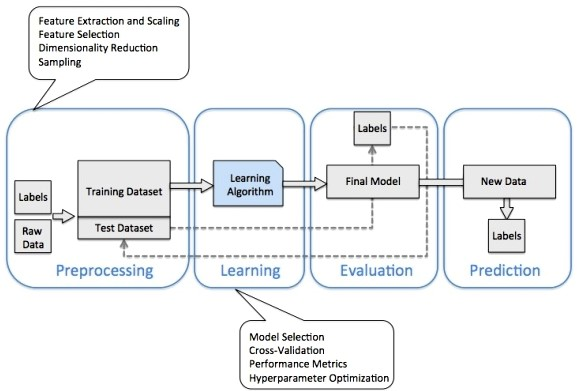
\includegraphics[scale=2.5]{methodology}
\caption{Proposed Methodology}
\label{figure:methodology}
\end{figure}


%
\section{Section(s)}
\label{methodology:section}
%
To provide a comprehensive understanding of the proposed methodology, break it down into easily digestible sections and subsections. Thoroughly explain each component and model selection, emphasizing the rationale behind the choices. Ensure clarity and accessibility throughout the document, making it easy for readers to grasp the presented concepts. Additionally, maintain proper citation practices, giving due credit when incorporating external resources, such as images or data, into the work.

You can generate an abbreviation and incorporate it into your text, for example: \gls{hstu}. Upon initial use, the complete meaning will be displayed. Subsequent references will only present the abbreviated form, such as \gls{hstu}.

Here are some examples of lists (bullet and numbered), tables, algorithms, and equations.

The following list consists of unordered bullet points.

\begin{itemize} \label{asd}
    \item \textbf{Label 1:} Some text...
    \item \textbf{Label 2:} Some text...
\end{itemize}

The following list consists of numbered points.

\begin{enumerate}
    \item \textbf{Label A:} Some text...
    \item \textbf{Label B:} Some text...
\end{enumerate}

Table \ref{table:results} displays randomly generated values for accuracy, precision, and F1-score as performance measures.

\begin{table}[H]
\centering
\caption{Results of Experiment}
\label{table:results}
\begin{tabularx}{0.8\linewidth}{@{ } X | *{3}{r} @{ }}
\toprule
\multirow{2}{*}{Model} & \multicolumn{3}{c}{Dataset} \\ 
        & Accuracy             & Precision              & F1      \\ 
\midrule
Model A & {93.57}  & {77.24}  & {95.36}           \\ 
Model B & {95.70}  & {60.51}  & {73.67}           \\ 
Model C & {56.46}  & {30.16}  & {54.47}           \\ 
Model D & {73.91}  & {37.70}  & {71.03}           \\ 
Model E & \textbf{98.41}  & \textbf{44.28}  & \textbf{76.91}  \\ 
Model F & {87.73}  & {43.17}  & {75.79}           \\
\bottomrule
\end{tabularx}
\end{table}

Algorithm \ref{algorithm:dividenumber} shows the steps for division of two numbers.

\begin{algorithm}[H]
\caption{ Divide Number ($num1, num2$)}
\label{algorithm:dividenumber}
\begin{algorithmic}[1]
\If{$num2 = 0$}
    \State return $Unknown$
\EndIf
\State $result = num1 / num2$
\State return $result$
\end{algorithmic}
\end{algorithm}

Equations (\ref{eq:one}) to (\ref{eq:three}) demonstrate the usage of the align construct for defining multiple equations.

\begin{align}
    (w^T x_i-\gamma)>=+1    \label{eq:one} \\
    (w^T x_i-\gamma)<=-1    \label{eq:two} \\
    (w^T x_i-\gamma)=0      \label{eq:three}
\end{align}

The formula for accuracy metric is given in (\ref{eq:accuracy}), where True Positives (\textit{TP}) are the correctly predicted positive cases, True Negatives (\textit{TN}) are the correctly predicted negative cases, False Positives (\textit{FP}) are the incorrectly predicted positive cases and False Negatives (\textit{FN}) are the incorrectly predicted negative cases.

\begin{equation}
\label{eq:accuracy}
accuracy = \frac{TP + TN}{TP + FP + TN + FN}
\end{equation}

\bigskip
You can also write in other languages by defining new font faces and uploading the \textit{ttf} file. For example, the following line is in Bengali: {\myfont{আমাদের সবাই একসাথে আগামী ভবিষ্যতের দিকে যাচ্ছি}}.


\newpage

\chapter{Results and Discussion}
\label{chapter:experiment}
% 
\section{Introduction}
\label{results:introduction}
% 
The results section presents the findings obtained from the research methods. It offers a clear, organized presentation of raw data, often utilizing tables, figures, or graphs to enhance understanding. The section focuses on facts and avoids interpretation or analysis, letting the data speak for itself. Rules for this section demand precision and objectivity. Results must be reported accurately, and any trends or patterns should be highlighted without bias. Every piece of data presented should directly relate to the research questions, ensuring relevance. Clarity is paramount; the information should be presented logically, guiding readers through the findings in a comprehensible manner, setting the stage for the subsequent analysis and discussion.


% 
\section{Evaluation and Discussion}
\label{results:evaluation}
% 
The evaluation and discussion section interprets the results within the context of the research questions and existing literature. It critically analyzes the findings, explores their implications, and assesses their significance. This section evaluates the study's strengths and limitations, addressing unexpected results and explaining their possible causes. Rules for this section demand depth and insight. It must demonstrate a clear understanding of the research's implications, relating the findings to the broader field of study. Critical thinking is essential; the discussion should offer reasoned interpretations, considering alternative explanations.

\newpage

\chapter{Conclusion and Future Work}
\label{chapter:conclusion}
% 
\section{Introduction}
\label{conclusion:introduction}
% 
The conclusion section provides a concise summary of the study's key findings, their significance, and their alignment with the research objectives. It offers closure, reaffirming the thesis statement and the contributions made to the field. Rules for this section require clarity and conciseness. It should restate the research problem and highlight the main outcomes, emphasizing their relevance. The conclusion must not introduce new ideas but rather synthesize existing ones, leaving a lasting impression on the reader. It should also address the study's limitations honestly. Lastly, the conclusion often suggests practical applications of the research and emphasizes its broader impact, leaving readers with a clear understanding of the study's significance.


% 
\section{Future Work}
\label{conclusion:future}
% 
The future works section outlines potential research directions and areas for further exploration based on the current study's findings and limitations. It suggests unresolved questions, methodologies that could enhance understanding, or applications that could arise from the research. The rules for this section necessitate insight and foresight. It should be specific, offering clear, well-defined suggestions for future researchers. Recommendations should be grounded in the study's conclusions and aimed at addressing its limitations or expanding upon its successes. Clarity is key; ideas should be presented logically, providing a roadmap for scholars interested in building upon the current research, encouraging a continuous scholarly discourse in the field.

\newpage
}

% .................................................................. %

% references
\pagestyle{plain}
\bibliographystyle{ieeetr}  % change to other styles if necessary
\addcontentsline{toc}{chapter}{References}
\bibliography{references}



% .................................................................. %



Appendix
Uncomment this part to add appendix
\newpage
\pagestyle{body}
\begin{appendices}
% 
\chapter{Some Appendix}
The contents...

\end{appendices}




\end{document}
